\begin{figure}[t]
  \subfloat[\mad assembly]{%
    \begin{minipage}[c]{0.95\columnwidth}%
      \centering
      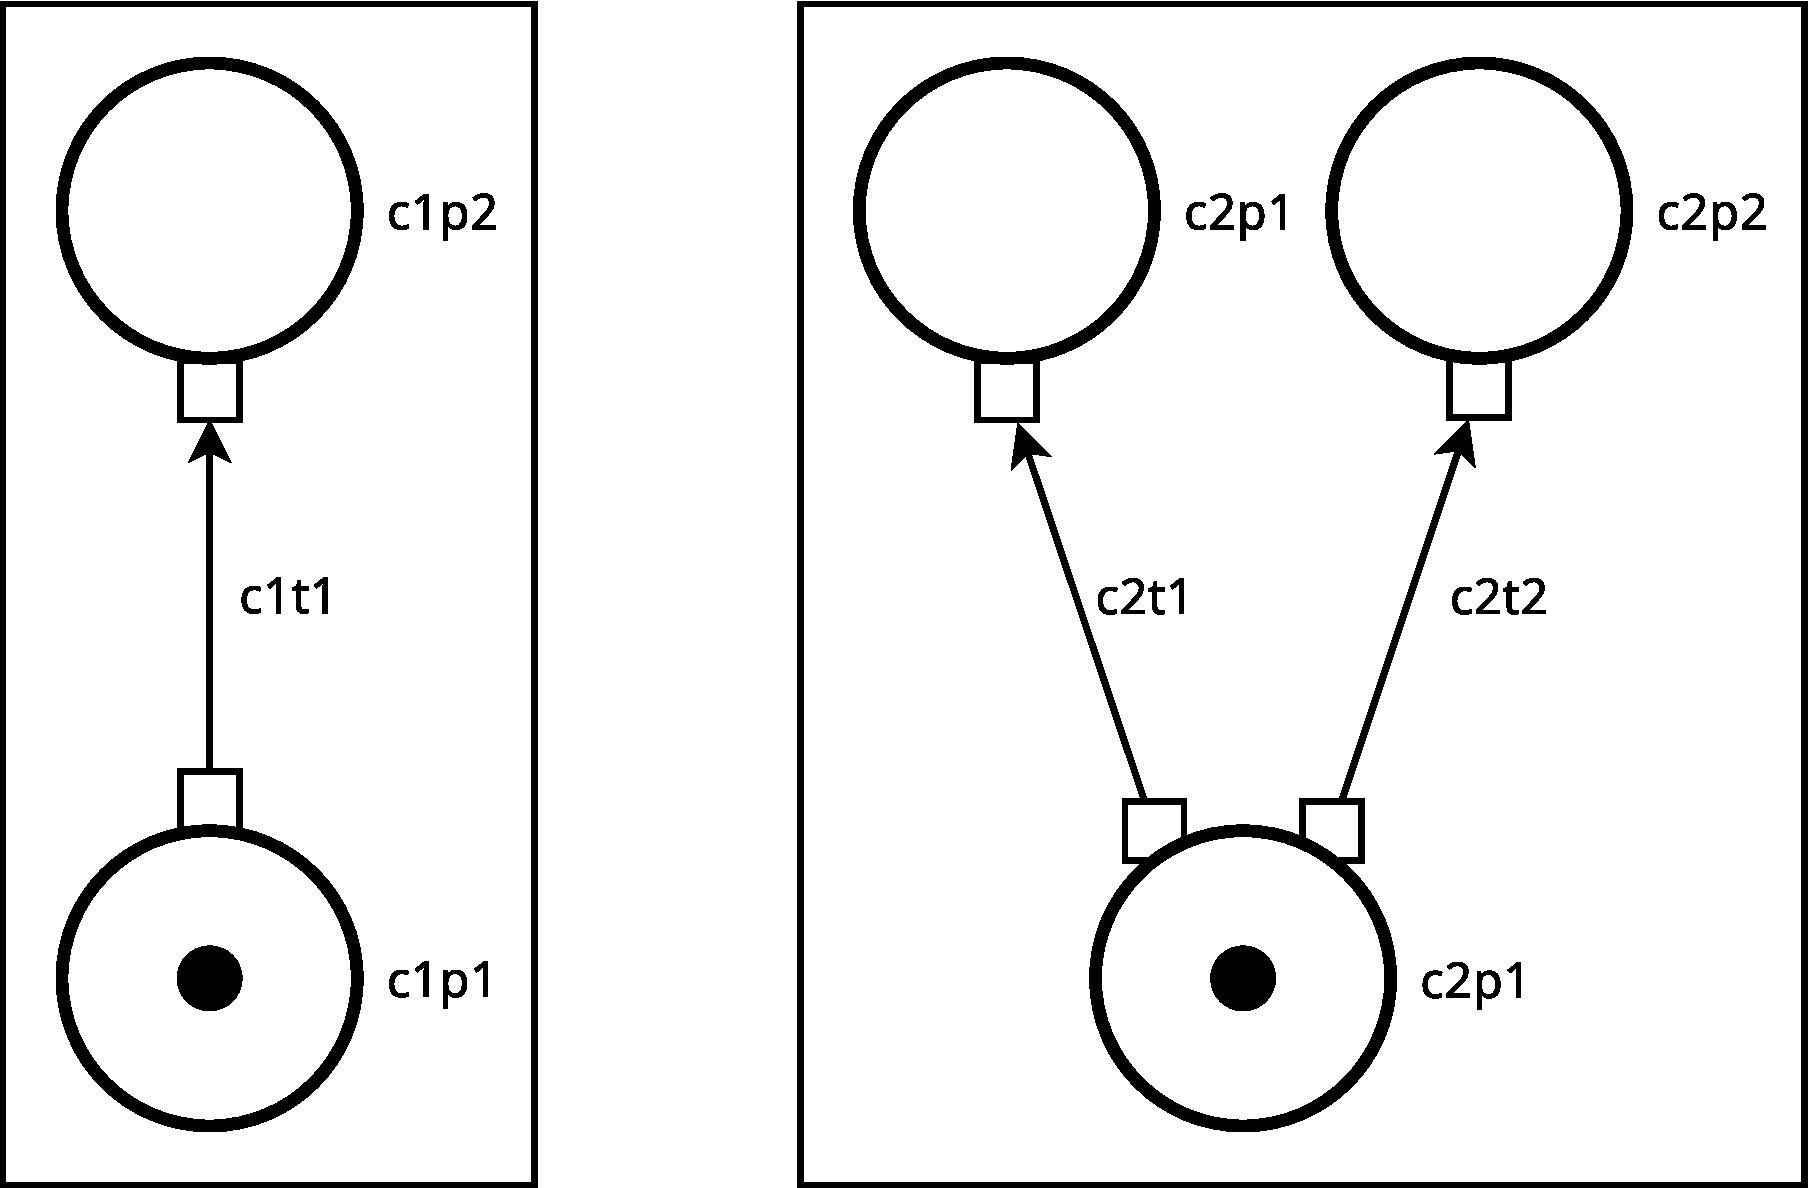
\includegraphics[scale=0.15]{images/perf_source_sink.pdf}
    \end{minipage}
  }
  \\
  
  \subfloat[Dependency graph]{%
    \fcolorbox{black!20}{white}{
      \begin{minipage}[c]{0.95\columnwidth}%
        \centering
        \begin{tikzpicture}[node distance=1.7cm]
          \node (c1p2l) [] {$v_\text{c1p2}^\text{leav}$};
          \node (c1p2) [below =15pt of c1p2l,yshift=-0.3cm] {$v_\text{p1p2}^\text{place}$};
          \node (c1t1e) [below =15pt of c1p2] {$v_\text{c1t1}^\text{end}$};
          \node (c1t1) [below =15pt of c1t1e] {$v_\text{c1t1}^\text{beg}$};
          \node (c1p1l) [below =15pt of c1t1] {$v_\text{c1p1}^\text{leav}$};
          \node (c1p1) [below =15pt of c1p1l] {$v_\text{c1p1}^\text{place}$};
          \node (c2p2) [right =35pt of c1p2] {$v_\text{c2p2}^\text{place}$};
          \node (c2p2l) [above =15pt of c2p2] {$v_\text{c2p2}^\text{leav}$};
          \node (c2t1e) [below =15pt of c2p2] {$v_\text{c2t1}^\text{end}$};
          \node (c2t1) [below =15pt of c2t1e] {$v_\text{c2t1}^\text{beg}$};
          \node (c2p1l) [below =15pt of c2t1, xshift=1.5cm] {$v_\text{c2p1}^\text{leav}$};
          \node (c2p1) [below =15pt of c2p1l] {$v_\text{c2p1}^\text{place}$};
          
          \node (c2p3) [right =35pt of c2p2] {$v_\text{c2p3}^\text{place}$};
          \node (c2p3l) [above =15pt of c2p3, yshift=0.3cm] {$v_\text{c2p3}^\text{leav}$};
          \node (c2t2e) [below =15pt of c2p3] {$v_\text{c2t2}^\text{end}$};
          \node (c2t2) [below =15pt of c2t2e] {$v_\text{c2t2}^\text{beg}$};
          
          \node (source) [below =15pt of c2p1, xshift=-1.8cm] {$v^\text{source}$};
          \node (sink) [above =20pt of c2p2l] {$v^\text{sink}$};
          
          \draw [->] (c1p1) -- (c1p1l) node[midway, right, scale=0.7] {$0$};
          \draw [->] (c1p2) -- (c1p2l) node[midway, right, scale=0.7] {$0$};
          \draw [->] (c2p1) -- (c2p1l) node[midway, right, scale=0.7] {$0$};
          \draw [->] (c2p2) -- (c2p2l) node[midway, right, scale=0.7] {$0$};
          \draw [->] (c2p3) -- (c2p3l) node[midway, right, scale=0.7] {$0$};
          \draw [->] (c1t1) -- (c1t1e) node[midway, right, scale=0.7] {$time(\text{c1t1})$};
          \draw [->] (c2t1) -- (c2t1e) node[midway, right, scale=0.7] {$time(\text{c2t1})$};
          \draw [->] (c2t2) -- (c2t2e) node[midway, right, scale=0.7] {$time(\text{c2t2})$};
          \draw [->] (c1p1l) -- (c1t1) node[midway, right, scale=0.7] {$0$};
          \draw [->] (c2p1l) -- (c2t1) node[midway, right, scale=0.7] {$0$};
          \draw [->] (c2p1l) -- (c2t2) node[midway, right, scale=0.7] {$0$};
          \draw [->] (c1t1e) -- (c1p2) node[midway, right, scale=0.7] {$0$};
          \draw [->] (c2t1e) -- (c2p2) node[midway, right, scale=0.7] {$0$};
          \draw [->] (c2t2e) -- (c2p3) node[midway, right, scale=0.7] {$0$};
          \draw [->] (source.west) to[bend left] node[midway, above, scale=0.7]{$0$} (c1p1.south);
          \draw [->] (source.east) to[bend right] node[midway, above, scale=0.7] {$0$}(c2p1.south);
          \draw [->] (c1p2) -- (sink) node[midway, right, scale=0.7] {$0$};
          \draw [->] (c2p2) to[bend right] node[midway, right, scale=0.7] {$0$}(sink);
          \draw [->] (c2p3) -- (sink) node[midway, right, scale=0.7] {$0$};
        \end{tikzpicture}
      \end{minipage}
    }
  }
  \caption{Transformation example from two components without ports to
    their equivalent dependency graph}
  \label{fig:source_sink_graph}
\end{figure}